\documentclass[10pt,a4paper]{article}
\usepackage[a4paper,margin=2.2cm]{geometry}
\usepackage{amsmath,amssymb}
\usepackage{graphicx}
\usepackage{booktabs}
\usepackage[hidelinks]{hyperref}
\usepackage{caption}
\captionsetup{font=small,labelfont=bf}
\usepackage{xcolor}
\graphicspath{{figures/}}
\emergencystretch=2em
\newcommand{\tabships}{
\begin{tabular}{lrrrrrrrr}\toprule
Ship & dry (t) & tank (t) & payload (t) & $m_0$ (t) & power (MW) & $a_{\min}$ (mm/s$^2$) & $a_{\max}$ (mm/s$^2$) & cr/day \\ \midrule
Freighter & 34.1 & 30 & 15.0 & 79.1 & 10.0 & 1.01 & 5.1 & 16 \\
Courier & 24.9 & 30 & 3.0 & 57.9 & 18.0 & 2.49 & 12.4 & 14 \\
Bulk tanker & 86.9 & 100 & 200.0 & 386.9 & 40.0 & 0.83 & 4.1 & 27 \\
Liner & 198.4 & 60 & 14.0 & 272.4 & 100.0 & 2.94 & 14.7 & 69 \\
Large liner & 885.5 & 300 & 65.0 & 1250.5 & 500.3 & 3.20 & 16.0 & 296 \\
\bottomrule\end{tabular}}
\newcommand{\tabsametime}{
\begin{tabular}{lrrrrrrrrr}\toprule
Ship & cases & min \% & max \% & mean \% & coast & sep.\ mean & sep.\ max & no B & branch \\
 & & \multicolumn{3}{c}{A's extra propellant over B} & of $T$ & \multicolumn{2}{c}{($10^6$ km)} & & \\ \midrule
Freighter & 222 & 0.04 & 16.9 & 0.80 & 14\% & 1.9 & 57.3 & 12 & 0 \\
Courier & 213 & 0.08 & 44.7 & 1.25 & 15\% & 5.2 & 504.5 & 19 & 2 \\
Bulk tanker & 221 & 0.02 & 9.7 & 0.96 & 15\% & 1.6 & 18.0 & 12 & 1 \\
Liner & 216 & 0.62 & 36.8 & 6.75 & 36\% & 10.4 & 307.8 & 18 & 0 \\
Large liner & 213 & 0.54 & 37.4 & 6.09 & 34\% & 9.4 & 295.0 & 21 & 0 \\
\bottomrule\end{tabular}}
\newcommand{\tabmintime}{
\begin{tabular}{lrrrrrrr}\toprule
Ship & departures & A flies & B flies & solver miss & min \% & max \% & mean \% \\
 & & \multicolumn{3}{c}{} & \multicolumn{3}{c}{A's extra time over B} \\ \midrule
Freighter & 234 & 234 & 234 & 16 & 0.0 & 66.9 & 7.34 \\
Courier & 234 & 234 & 234 & 25 & 0.0 & 52.3 & 4.94 \\
Bulk tanker & 234 & 234 & 234 & 15 & 0.0 & 48.3 & 2.24 \\
Liner & 234 & 234 & 234 & 22 & 0.0 & 33.9 & 2.63 \\
Large liner & 234 & 234 & 234 & 25 & 0.0 & 58.5 & 2.53 \\
\bottomrule\end{tabular}}
\newcommand{\tabeconomic}{
\begin{tabular}{lrrrrrrr}\toprule
Ship & cases & min \% & max \% & mean \% & $T_A/T_B$ & fuel$_A$/fuel$_B$ & solver miss \\
 & & \multicolumn{3}{c}{A's extra trip cost over B} & \multicolumn{2}{c}{mean, B solved} & \\ \midrule
Freighter & 234 & 0.00 & 6.25 & 0.81 & 1.009 & 1.037 & 21 \\
Courier & 234 & 0.00 & 2.87 & 1.41 & 0.996 & 1.114 & 25 \\
Bulk tanker & 234 & 0.00 & 4.44 & 1.23 & 0.998 & 1.094 & 43 \\
Liner & 234 & 0.00 & 31.22 & 2.81 & 1.022 & 1.077 & 31 \\
Large liner & 234 & 0.00 & 30.43 & 3.01 & 1.026 & 1.080 & 28 \\
\bottomrule\end{tabular}}
\newcommand{\tabtanks}{
\begin{tabular}{lrrrrrrrrr}\toprule
Ship & \multicolumn{4}{c}{A: best tank} & \multicolumn{4}{c}{B: best tank} & differ \\
 & 50\% & 100\% & 150\% & 200\% & 50\% & 100\% & 150\% & 200\% &  \\ \midrule
Freighter & 189 & 42 & 2 & 1 & 189 & 42 & 2 & 1 & 10 \\
Courier & 217 & 11 & 3 & 3 & 220 & 8 & 2 & 4 & 5 \\
Bulk tanker & 171 & 58 & 4 & 1 & 186 & 42 & 5 & 1 & 21 \\
Liner & 41 & 110 & 55 & 28 & 56 & 105 & 56 & 17 & 49 \\
Large liner & 58 & 107 & 63 & 6 & 75 & 117 & 41 & 1 & 52 \\
\bottomrule\end{tabular}}
\newcommand{\tabtiming}{
\begin{tabular}{lrrrrrrr}\toprule
 & solved & median & mean & p90 & p99 & max & over 100\,ms \\ \midrule
Earliest arrival, ideal engine & 240/240 & 2.7 & 5.2 & 11.1 & 52 & 69 & 0 \\
Earliest arrival, A & 240/240 & 5.4 & 20.3 & 57.4 & 238 & 366 & 12 \\
Earliest arrival, B & 237/240 & 9.3 & 243.7 & 136.3 & 5760 & 21909 & 26 \\
One B solve, from the ideal seed & 237/240 & 1.1 & 9.4 & 3.9 & 206 & 360 & 6 \\
One B solve, warm (neighbouring $T$) & 237/240 & 0.5 & 1.7 & 1.0 & 4 & 175 & 1 \\
B search that fails & 3 &  & 69397 &  &  & 112745 &  \\
\bottomrule\end{tabular}}
\newcommand{\tabtuning}{
\begin{tabular}{lrrrrrr}\toprule
Variant & solved & A flies: solved & median & mean & mean & propagations \\
 & & & \multicolumn{2}{c}{ms, solved} & ms, failed & mean \\ \midrule
default & 457/720 & 350/399 & 1.7 & 50 & 1169 & 228 \\
no smoothing fallback & 449/720 & 343/399 & 1.6 & 15 & 52 & 134 \\
finite-difference Jacobian & 435/720 & 330/399 & 2.7 & 29 & 289 & 414 \\
DOPRI5 (1e-10) & 459/720 & 353/399 & 2.5 & 67 & 611 & 221 \\
DOP853 at 1e-9 & 451/720 & 344/399 & 1.6 & 60 & 1208 & 239 \\
fallback smoothing down to 1e-3 & 456/720 & 349/399 & 2.0 & 54 & 1205 & 229 \\
band in one step & 458/720 & 352/399 & 1.1 & 43 & 1230 & 233 \\
no secant predictor & 407/720 & 300/399 & 2.0 & 95 & 1151 & 191 \\
\bottomrule\end{tabular}}
\newcommand{\sameN}{1085}
\newcommand{\sameMin}{0.02}
\newcommand{\sameMean}{3.1}
\newcommand{\sameMedian}{0.9}
\newcommand{\sameMax}{45}
\newcommand{\sameNoB}{82}
\newcommand{\sameBranch}{3}
\newcommand{\timeMean}{3.9}
\newcommand{\timeMax}{67}
\newcommand{\timeMiss}{103}
\newcommand{\onlyB}{0}
\newcommand{\nBase}{1170}
\newcommand{\nAll}{4680}
\newcommand{\econMean}{1.85}
\newcommand{\econMax}{31.2}
\newcommand{\econMiss}{148}
\newcommand{\bSolves}{262\,044}
\newcommand{\bFailPct}{18.5}
\newcommand{\checkMedianM}{20}
\newcommand{\checkNinetyNine}{7}
\newcommand{\checkBad}{1}
\newcommand{\timingN}{240}


\title{Flying inside the exhaust band\\[2pt]\large Ideal-then-throttle versus banded-optimal transfers for the SpaceTrains plasma fleet}
\author{SpaceTrains trajectory study}
\date{October 2026}

\begin{document}
\maketitle

\begin{abstract}
SpaceTrains plans its plasma ships with an \emph{ideal} constant-power drive whose exhaust speed may take any value.
The game's drives are confined to an exhaust band of 50--250\,km/s. Two ways of respecting the band are compared on
the game's five plasma hulls (four tank sizes each), eight heliocentric routes and 18--36 departure angles per route. \textbf{A}~plans the
ideal path and flies it inside the band, throttling at 250\,km/s where the path asks for less thrust than the drive
gives at full power. \textbf{B}~plans the true optimum inside the band, with a new solver written for this study.
At the same transfer time A burns a median 0.9\% (mean \sameMean\%, maximum \sameMax\%) more propellant than B.
The cargo hulls lose about 1\%. The liners lose 6--7\%, because their power-to-mass ratio puts their thrust at
250\,km/s above what most of the path asks for. On a full tank B arrives \timeMean\% earlier on average, and up to
\timeMax\% on short inner-system windows. The cheapest trip costs \econMean\% more with A on average, up to \econMax\%
for the liners. B's paths coast for 15\% (cargo) to 35\% (liners) of the trip and leave A's path by
$10^6$--$10^8$\,km on the outer legs. The tank choice changes on about one departure in five. B solves in about
1\,ms when it converges. It still fails on 18\% of the fixed-time problems in the sweeps, and a failing search can
take a minute. The recommendation is to keep A as the game's planner. B could later serve as an optional,
time-boxed refinement for liners.
\end{abstract}

\section{The question}

A constant-power drive with jet power $P$ trades thrust for exhaust speed: at full power the thrust acceleration is
$a = 2P/(m v_e)$. With $v_e$ free, minimum propellant is minimum $\int a^2\,dt$, the optimal path does not depend
on the ship's mass, and one atlas of paths serves every ship. This is how the game plans today.

The game's drives have an exhaust band $[v_{\min}, v_{\max}] = [50, 250]$\,km/s. Writing $s = 2P/m$, at full power
the band allows $a \in [a_{\min}, a_{\max}] = [s/v_{\max}, s/v_{\min}]$. Below $a_{\min}$ the drive can only run at
$v_{\max}$ and part power (or pulse at full power, the same on average). Above $a_{\max}$ it cannot go at all.

\begin{description}
\item[A: plan ideal, fly banded.] Plan the ideal path. Fly it exactly, throttled at $v_{\max}$ where $a < a_{\min}$.
  Reject it where $a > a_{\max}$. The path and its boundary conditions are unchanged; only the propellant grows.
  This is what the branch \texttt{feature/exhaust\_band} does in the game.
\item[B: plan banded, fly banded.] Solve the minimum-propellant problem with the band as a constraint, and fly that.
\end{description}

Both are exact in the sense that the ship arrives where and when the plan says. A is never better than B: B is the
optimum among all controls the drive can fly, and A's control is one of them. The questions are how much A loses
(propellant at a fixed time, time on a fixed tank, cost of the trip), how different the paths are, whether the
choice of tank changes, and whether B is fast enough for the game.

\section{Model}

Planar two-body motion about the Sun, normalised units ($\mu = 1$, length 1\,AU, speed 29.78\,km/s, time
58.13\,days). The state is $(\mathbf r, \mathbf v, s)$ with
\begin{equation}
\dot{\mathbf r} = \mathbf v,\qquad \dot{\mathbf v} = -\mathbf r/r^3 + a\,\hat{\mathbf u},\qquad
\dot s = l(a) = a\,\max(a, a_{\min}),\qquad a_{\min} = s/v_{\max},\quad 0 \le a \le a_{\max} = s/v_{\min}.
\end{equation}
Inside the band $l = a^2$ (the ideal drive). Throttled at $v_{\max}$ it is $l = a\,a_{\min}$, which is
$\dot m = -m a/v_{\max}$, the rocket equation at $v_{\max}$. The final mass is $m_f = 2P/s(T)$, so minimum propellant
is minimum $s(T)$. A ship enters only through $s_0 = 2P/m_0$ and its band. The ideal solution is the case
$v_{\min} = 0$, $v_{\max} = \infty$, where $s(T) - s_0 = \int a^2 dt$ is the effort the game's atlas stores.

\subsection{Optimal control inside the band}

With the primer $\mathbf p = -\boldsymbol\lambda_v/2$ (so that the ideal thrust is $\mathbf a = \mathbf p$, the game
solver's convention), $\mathbf w = \dot{\mathbf p}$, $\dot{\mathbf w} = G(\mathbf r)\,\mathbf p$, and the costate
$\lambda_s$ of $s$, Pontryagin's principle asks the thrust to point along $\mathbf p$ and its size to minimise
$-2|\mathbf p|\,a + \lambda_s\,l(a)$ on $[0, a_{\max}]$. With $q = |\mathbf p|/\lambda_s$:

\begin{center}
\begin{tabular}{llll}\toprule
arc & condition & thrust & $\dot\lambda_s$ \\ \midrule
coast & $q \le a_{\min}/2$ & $0$ & $0$ \\
ceiling & $a_{\min}/2 < q < a_{\min}$ & $a_{\min}$ (full power, $v_{\max}$) & $(2|\mathbf p| - 2\lambda_s a_{\min})/v_{\max}$ \\
inside the band & $a_{\min} \le q < a_{\max}$ & $q$ & $0$ \\
floor & $q \ge a_{\max}$ & $a_{\max}$ (full power, $v_{\min}$) & $(2|\mathbf p| - 2\lambda_s a_{\max})/v_{\min}$ \\
\bottomrule\end{tabular}
\end{center}

Below the ceiling the cost is linear in $a$, so the optimum never throttles: it burns at full power and $v_{\max}$
or coasts, and the switch between them is a jump in thrust. The costates are homogeneous, so $\lambda_s(0) = 1$
fixes their scale. The unknowns are then $(\mathbf p_0, \mathbf w_0)$, as for the ideal problem. With no band,
$\lambda_s \equiv 1$ and the ideal primer solves the banded problem as it is. The Hamiltonian
$H = 2\mathbf w\cdot\mathbf v - 2\mathbf p\cdot(\mathbf g + \mathbf a) + \lambda_s l(a)$ is constant along an
extremal, which the tests use as a check.

\section{The solver}

\texttt{src/variable\_isp/BandedTransfer.\{hpp,cpp\}} (namespace \texttt{variable\_isp::banded}) is separate from the
game's ideal solver. It uses only that solver's public types and its \texttt{solve\_transfer} for the ideal seed.
It is built as its own library, which only its test and the study driver link.

\paragraph{Propagation.} Adaptive DOP853 (or DOPRI5), on one arc at a time. When the arc at the end of an accepted
step differs from the arc at its start, the switch is located on the boundary function (Illinois iterations on
trial steps in the old arc's flow). The step is cut there and the new arc continues. The sensitivities of the end
state to $(\mathbf p_0, \mathbf w_0)$ come from forward-mode dual numbers, four directions in one propagation. At a
switch where the thrust jumps (coast/ceiling), the saltation term
$\delta\mathbf x^+ = \delta\mathbf x^- + (\mathbf f^- - \mathbf f^+)\,\delta t^*$ carries the moving switch time into
them.

\paragraph{Fixed-time solve.} Damped Newton on the four rendezvous residuals. It works in up to three stages:
\begin{enumerate}
\item From a warm start (a neighbouring time or departure), Newton directly at the full band.
\item Otherwise continuation in band tightness: the band at $v_{\max}/\lambda$ and $\lambda v_{\min}$, $\lambda$ from
  0 (the ideal solution) to 1, adaptive steps and a secant predictor.
\item If that fails (typically when a coast arc is born on the way: there the end state depends on the unknowns
  through a square root and Newton stalls), the same continuation on a smoothed problem. The ceiling cost
  $a\max(a, a_{\min})$ is replaced by $a\cdot\tfrac12\big(a + a_{\min} + \sqrt{(a-a_{\min})^2 + \varepsilon^2 a_{\min}^2}\big)$,
  whose exact minimiser is a continuous control. Then $\varepsilon$ goes from 0.3 down to $10^{-2}$, and an exact
  polish ($\varepsilon = 0$) follows. When a switch grazes its boundary the exact problem is ill-conditioned; the
  smoothed plan is then kept. Its intermediate thrust is throttling at $v_{\max}$, so it is a flyable,
  near-optimal plan, and its propellant is integrated with the drive's true flow.
\end{enumerate}
A converged extremal that burns more than A at the same time is on another branch and is rejected.

\paragraph{Tuning.} Variants were run on a tuning set: the five hulls, the eight routes, six departures each, and
transfer times of 0.25, 0.5 and 1 Hohmann times, 720 cases in all (Table~\ref{tab:tuning}). Where several variants converge they land on the same extremal. What differs is how often they converge and at
what cost. ``A flies'' marks the 399 cases where the ideal path stays under the 50\,km/s floor, so a banded
solution certainly exists. In the other 321, A cannot fly at all and B may or may not exist.
\begin{itemize}
\item \textbf{Speed.} A solve that converges usually takes 1--3\,ms (the median). The mean is pulled up by a tail
  of hard cases.
\item \textbf{Jacobian.} Dual numbers beat finite differences on both counts: 20 more cases, and half the
  propagations. A finite-difference step across a switch sees the switch move and returns a poor Jacobian.
\item \textbf{Integrator.} DOP853 at $10^{-10}$ is kept. DOPRI5 solves three more cases but is 50\% slower per
  solve. A looser $10^{-9}$ loses six cases to noisy switch times.
\item \textbf{Continuation.} The secant predictor matters most: without it 50 cases are lost. Going to the full
  band in one step is as good on this set, because most cases need no continuation at all. The adaptive path is
  kept for the cases that do.
\item \textbf{Smoothing fallback.} It adds 7 cases (2\%), but it is expensive: a case that fails anyway costs about
  1.2\,s before giving up, against 50\,ms without the fallback. The study keeps it for coverage. A game would not;
  it would fail fast and fly A instead (Section~\ref{sec:game}).
\end{itemize}
The cases still unsolved where A flies (49 of 399) are mostly long outer transfers near the Hohmann time. Their
optimum is dominated by coasting, and coast arcs are born and die along the continuation path. On the other side,
B solves 107 cases in which the ideal path breaks the floor and A cannot fly.

\begin{table}[h]\centering\small
\caption{Solver variants on the tuning set (cases where the ideal problem solves). One process per variant, eight
in parallel, so absolute times are indicative; Table~\ref{tab:timing} has the one-thread timings.}
\label{tab:tuning}
\tabtuning
\end{table}

\paragraph{Validation.} \texttt{tests/banded\_transfer\_test.cpp}:
\begin{itemize}
\item \textbf{No band, or a band the path never touches:} the ideal primer meets the target and
  $s(T) - s_0$ equals the ideal effort (to $10^{-8}$).
\item \textbf{Jacobian:} the dual-number Jacobian across switches matches finite differences.
\item \textbf{Free-space rest-to-rest with a ceiling:} the solver finds burn, coast, burn, with switch times
  ($10^{-7}$) and final mass ($10^{-9}$) equal to the closed form. The closed form is
  $u = 1 - e^{-\Delta v/v_{\max}}$, $t_1 = u v_{\max}^2/s_0$, $t_2 = (1-u)t_1$, $s(T) = s_0/(1-u)^2$.
\item \textbf{Throttled ideal path:} it matches the rocket equation at $v_{\max}$.
\item \textbf{Hamiltonian:} constant across switches.
\item \textbf{Heliocentric leg:} B never burns more than A, and a warm start from the answer converges at once.
\end{itemize}

\section{Study setup}

\paragraph{Ships.} The five plasma hulls of the game (Table~\ref{tab:ships}), each with its four tank variants
(50, 100, 150 and 200\% of the standard tank). Freighters and tankers carry a full hold at 100\,kg a unit. Liners
carry full berths, at 100\,kg a passenger with luggage plus 100 days of consumables. The band is 50--250\,km/s for
all; police ships are out of scope. The Luna ferry only flies planet-system spirals and is left out.

\begin{table}[h]\centering\small
\caption{The plasma hulls at their standard tanks, fully loaded. $a_{\min}$ and $a_{\max}$ are the thrust
accelerations at full power and 250 or 50\,km/s, at departure. The daily cost is the game's capital charge plus crew
and life support.}
\label{tab:ships}
\setlength\tabcolsep{4pt}\tabships
\end{table}

\paragraph{Legs.} Earth$\to$Mars, Mars$\to$Earth, Earth$\to$Venus, Earth$\to$Mercury, Earth$\to$Ceres,
Mars$\to$Ceres, Earth$\to$Jupiter and Jupiter$\to$Saturn, on the game's Kepler orbits (real eccentricities). The
departures are spread evenly over one synodic period: 36 on the first five routes, 18 on the last three, where each
departure costs more to compute. That makes 234 departures; with five hulls and four tank sizes, \nAll{} cases. The phase angle is the destination's lead over the origin at departure.
The ship leaves on the origin planet's heliocentric state and meets the destination's: the planet-system spirals
are not part of the heliocentric leg, as in the game. Closest solar pass 0.1\,AU.

\paragraph{B where its solver misses.} B's optimum can never be worse than A, so wherever the solver returns a
worse answer, or none, the planner flies A's plan instead. The tables count these cases as \emph{solver misses}.
Their excess is zero, which understates B's advantage a little.

\paragraph{What is compared.} For each ship and departure, on a log grid of 44 transfer times
($0.05$--$4$ Hohmann times, at least 20 days, at most two years past Hohmann):
\begin{enumerate}
\item \textbf{Same time:} the propellant of A and B at A's shortest feasible time (B's when only B flies), and
  the largest distance between the two paths along the way.
\item \textbf{Shortest time on a full tank:} the earliest arrival each approach can fly with the standard tank
  (10\% reserve), refined by bisection to 0.02\%.
\item \textbf{Cheapest trip:} propellant bought at the game's fuel price plus the ship's daily cost times the
  transfer time. The ship tanks 1.1 times the burn, solved self-consistently since the load changes $s_0$. The
  optimum over the grid is refined by a parabola. Done for every tank variant, which gives the best tank per
  approach.
\end{enumerate}
The \emph{error} of A is its excess over B: propellant at the same time, time on the same tank, cost of the
cheapest trip. B is the reference.

\section{Results}

\paragraph{Same transfer time.} Table~\ref{tab:same} and Figure~\ref{fig:fuel} compare the propellant at A's shortest
full-tank time. That is the point where the band binds hardest on A's plan; at longer times both approaches burn
less and the gap narrows (Figure~\ref{fig:curves}). Over \sameN{} pairs A's excess is between \sameMin\% and
\sameMax\%, with a median of \sameMedian\% and a mean of \sameMean\%.
\begin{itemize}
\item \textbf{Cargo hulls} (freighter, courier, bulk tanker) lose about 1\% on average. Their full-power thrust at
  250\,km/s (0.8--2.5\,mm/s$^2$) is below what the path asks for most of the way, so A throttles only briefly
  around the mid-course minimum.
\item \textbf{Liners} have 3\,mm/s$^2$ at the ceiling. They throttle for much of a transfer, and A loses 6--7\% on
  average and up to 37\%.
\item \textbf{Outer legs} (Earth$\to$Jupiter, Jupiter$\to$Saturn) are the worst, at about 10\% on average. Their
  thrust profile is low for months.
\end{itemize}
In \sameNoB{} cases B did not converge at that time. In \sameBranch{} cases B found a cheaper path than the ideal
engine itself: a different local optimum, left out of the statistics.

\begin{table}[h]\centering\small
\caption{Same transfer time (A's shortest on a full tank). A's excess propellant over B, the share of the transfer
B spends coasting, and the largest distance between the two paths. ``no B'': the solver did not converge.
``branch'': B landed on a different, cheaper local optimum.}
\label{tab:same}
\tabsametime
\end{table}

\begin{figure}[h]\centering
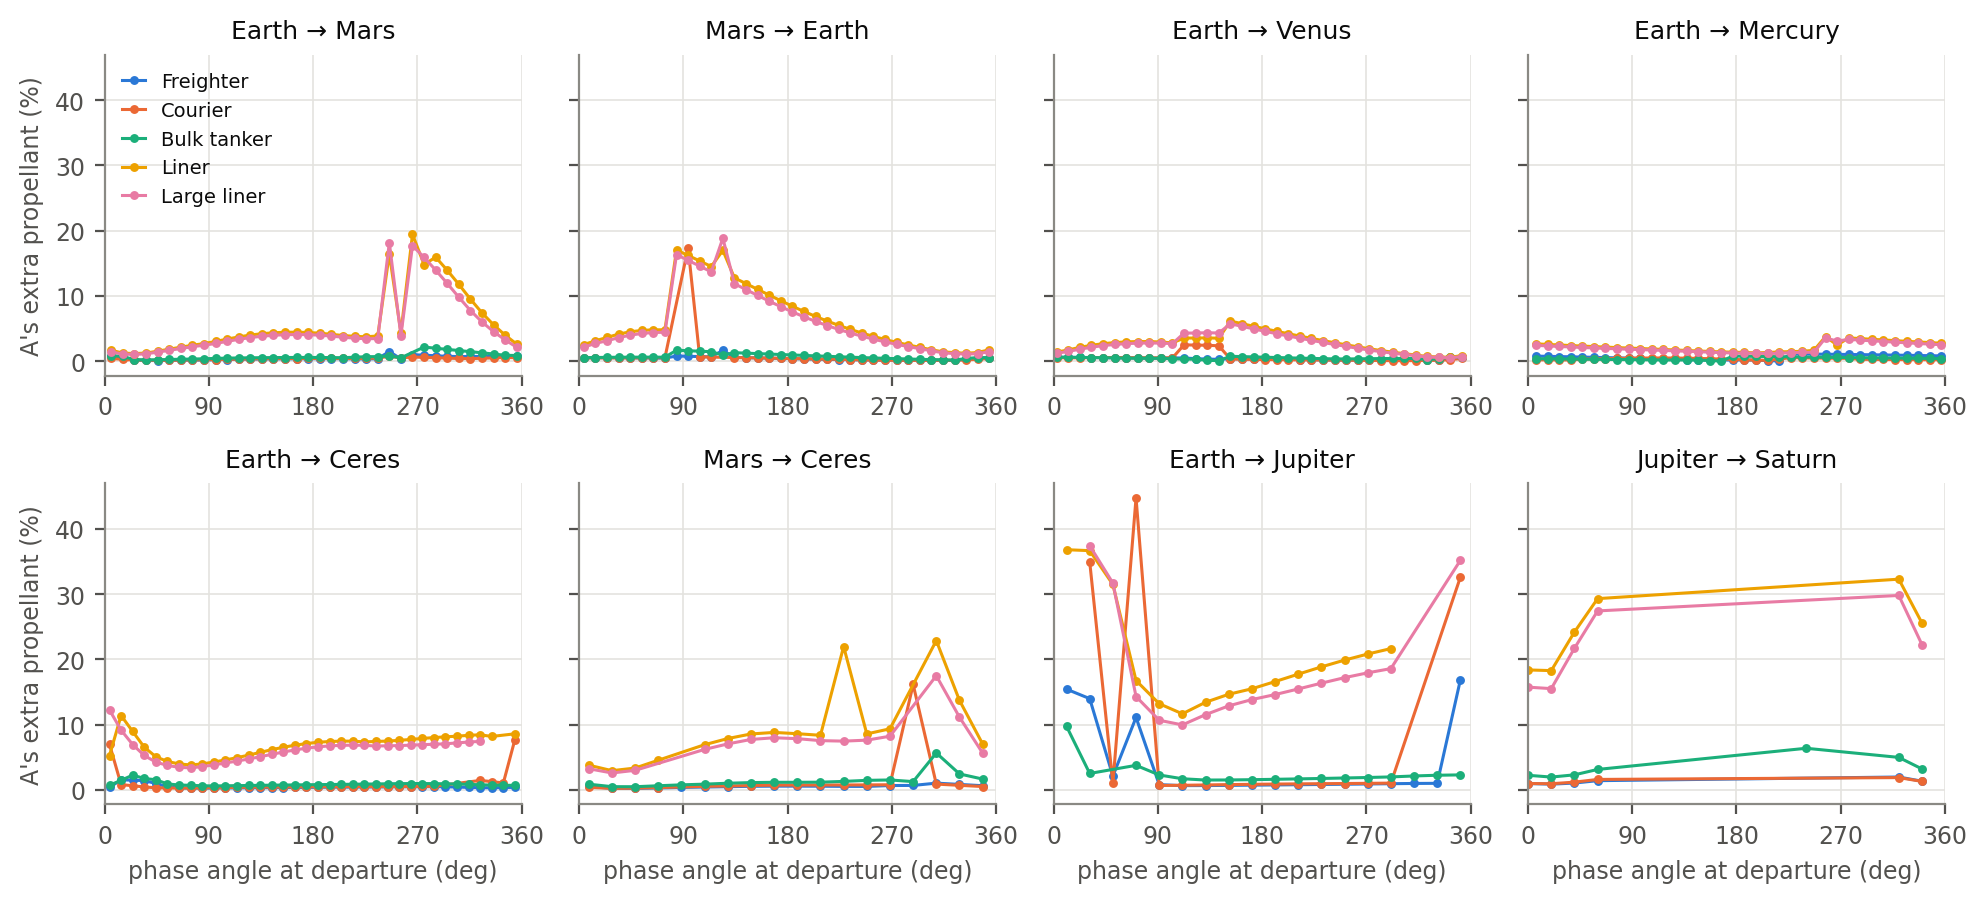
\includegraphics[width=\textwidth]{fuel_by_phase}
\caption{A's extra propellant over B at the same transfer time, against the departure phase angle. The liners'
peaks are departures where the shortest time is long and the thrust stays low through the middle of the trip.}
\label{fig:fuel}
\end{figure}

\begin{figure}[h]\centering
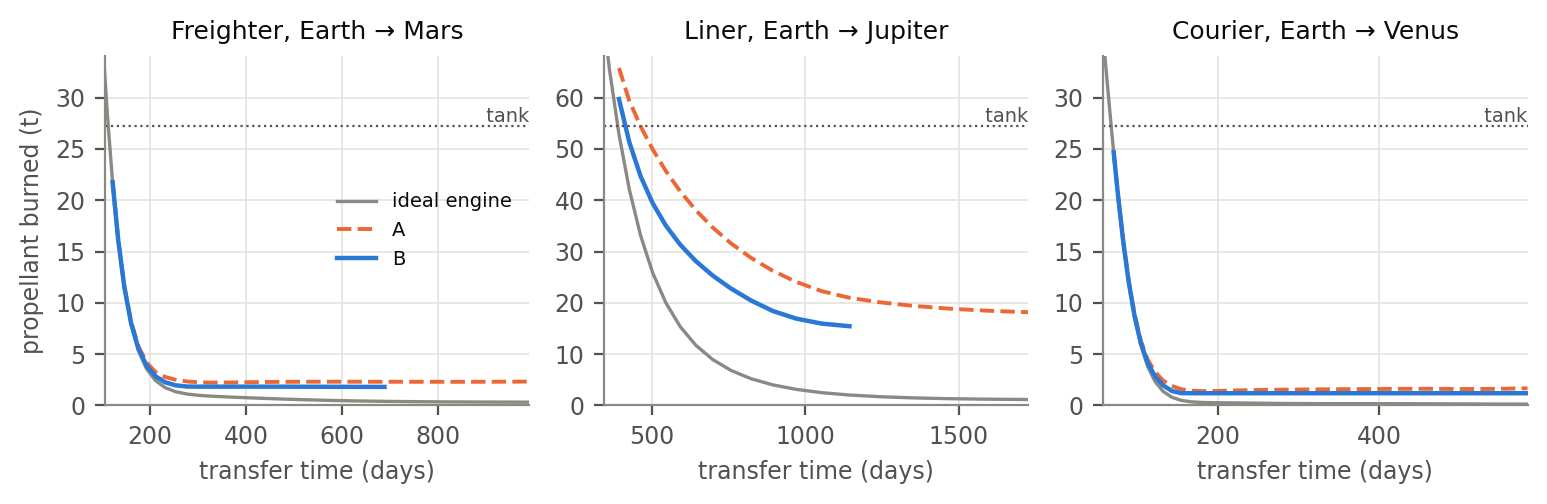
\includegraphics[width=\textwidth]{fuel_curves}
\caption{Propellant against transfer time for one departure each: ideal engine (lower bound), A and B. Where B's curve
ends, its solver stopped converging (long, coast-dominated transfers). The dotted line is the standard tank
less the reserve.}
\label{fig:curves}
\end{figure}

\paragraph{Shape of the optimum.} B is bang--coast--bang wherever A throttles. Inside the band it follows the ideal
thrust law. Where the ideal thrust drops below the ceiling, B burns at full power and 250\,km/s, then coasts, then
burns again (Figures~\ref{fig:paths-inner} and~\ref{fig:paths-outer}). Coasting takes 14--15\% of a cargo
transfer and 34--36\% of a liner transfer (Figure~\ref{fig:arcs}). The floor is almost never touched (below 0.1\%
of the time in every case): at the times compared here the ideal thrust exceeds the floor only near the ends, and
B's continuation turns those into slightly longer ceiling burns.

\begin{figure}[h]\centering
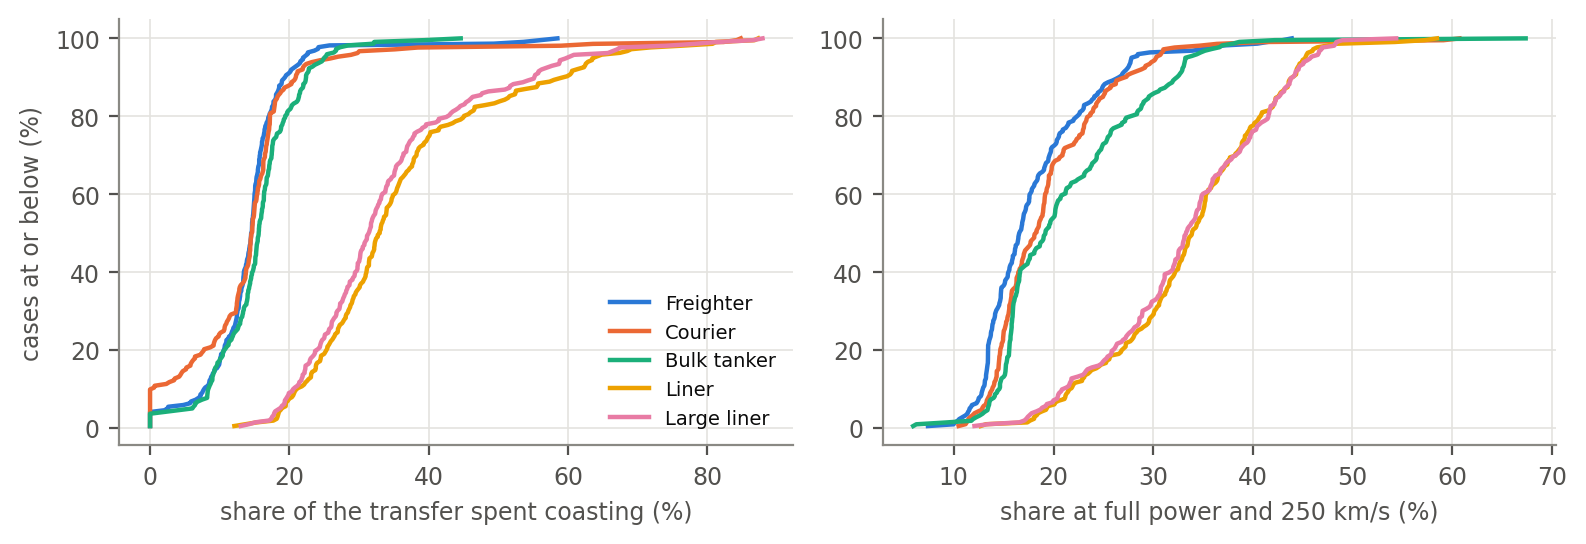
\includegraphics[width=0.85\textwidth]{arc_shares}
\caption{Distribution over departures of the share of the transfer B spends coasting and at full power on the
ceiling, at the same time as in Table~\ref{tab:same}.}
\label{fig:arcs}
\end{figure}

\paragraph{Trajectory differences.} Both plans start and end on the same states, so the difference is in between.
On the inner routes the paths separate by a median of 0.4--1.2 million km (up to 46 million km for the liners). On
the outer routes the median is 2--9 million km. The largest separations, 100--500 million km, are two-year
Jupiter transfers in which B's long coast puts it on a visibly different ellipse
(Figure~\ref{fig:sep}). In the game these are not small corrections: a B ship on a map would fly a different line
from the one A plans.

\begin{figure}[h]\centering
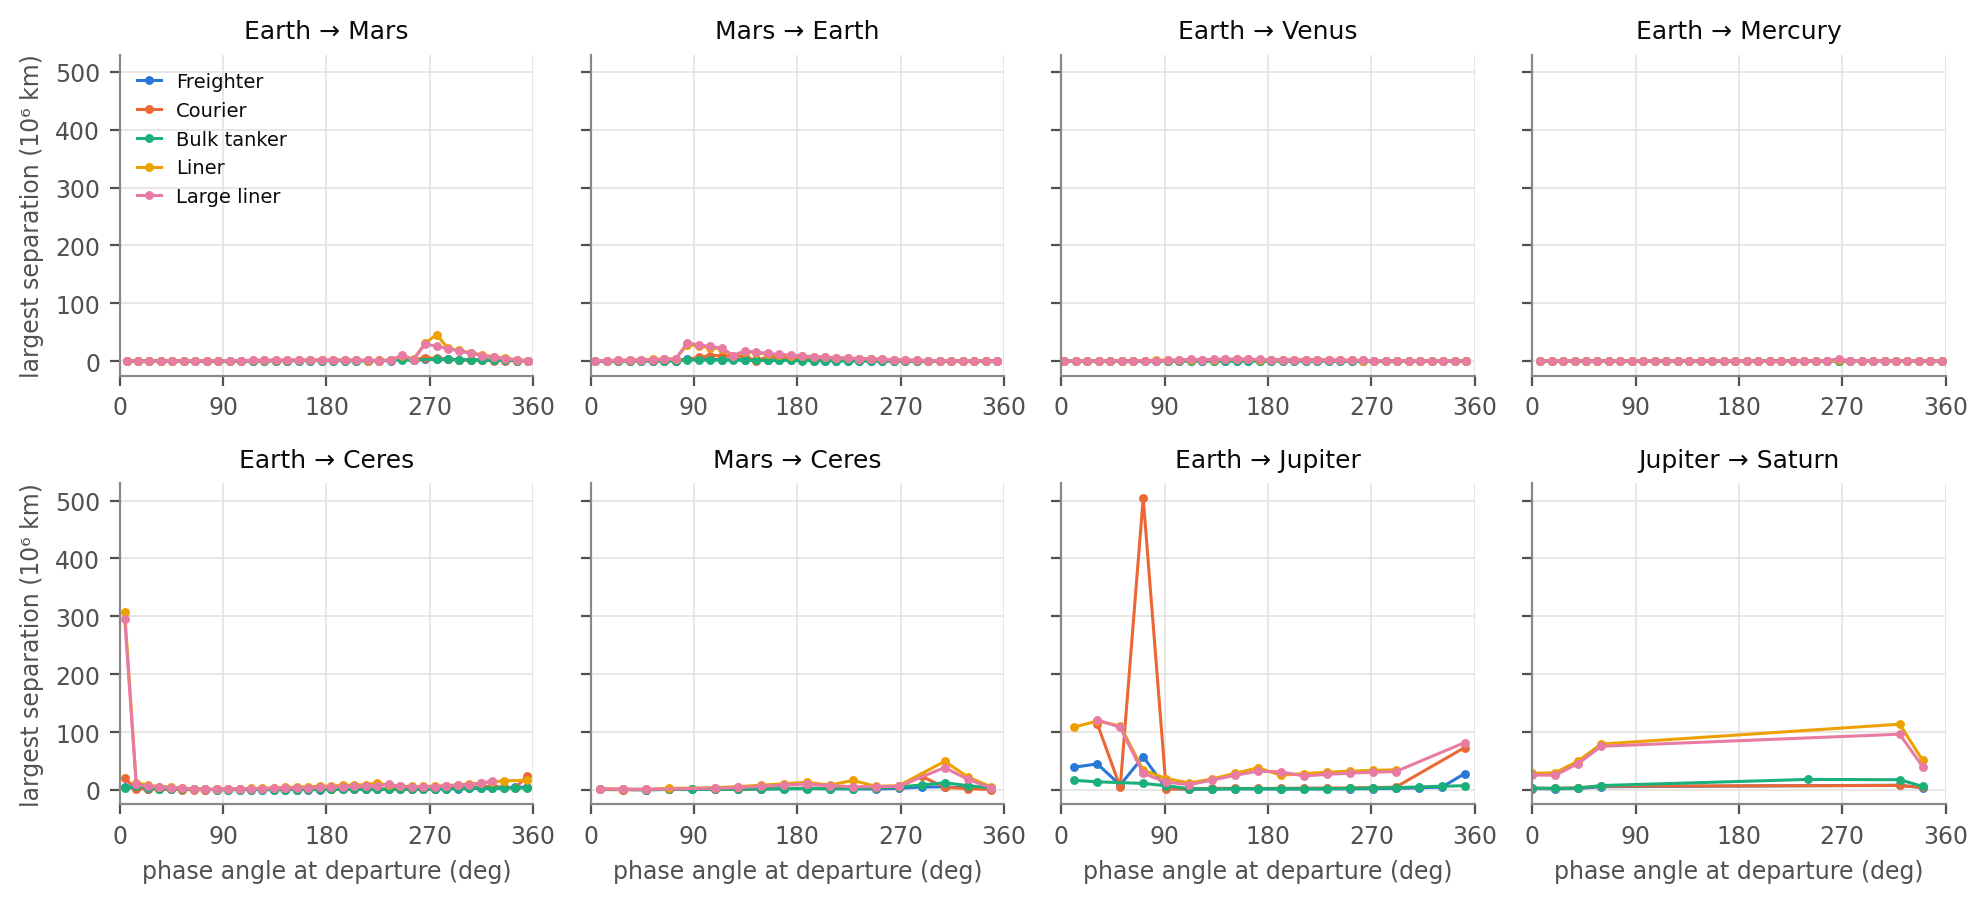
\includegraphics[width=\textwidth]{separation_by_phase}
\caption{Largest distance between A's and B's paths at the same transfer time.}
\label{fig:sep}
\end{figure}

\begin{figure}[p]\centering
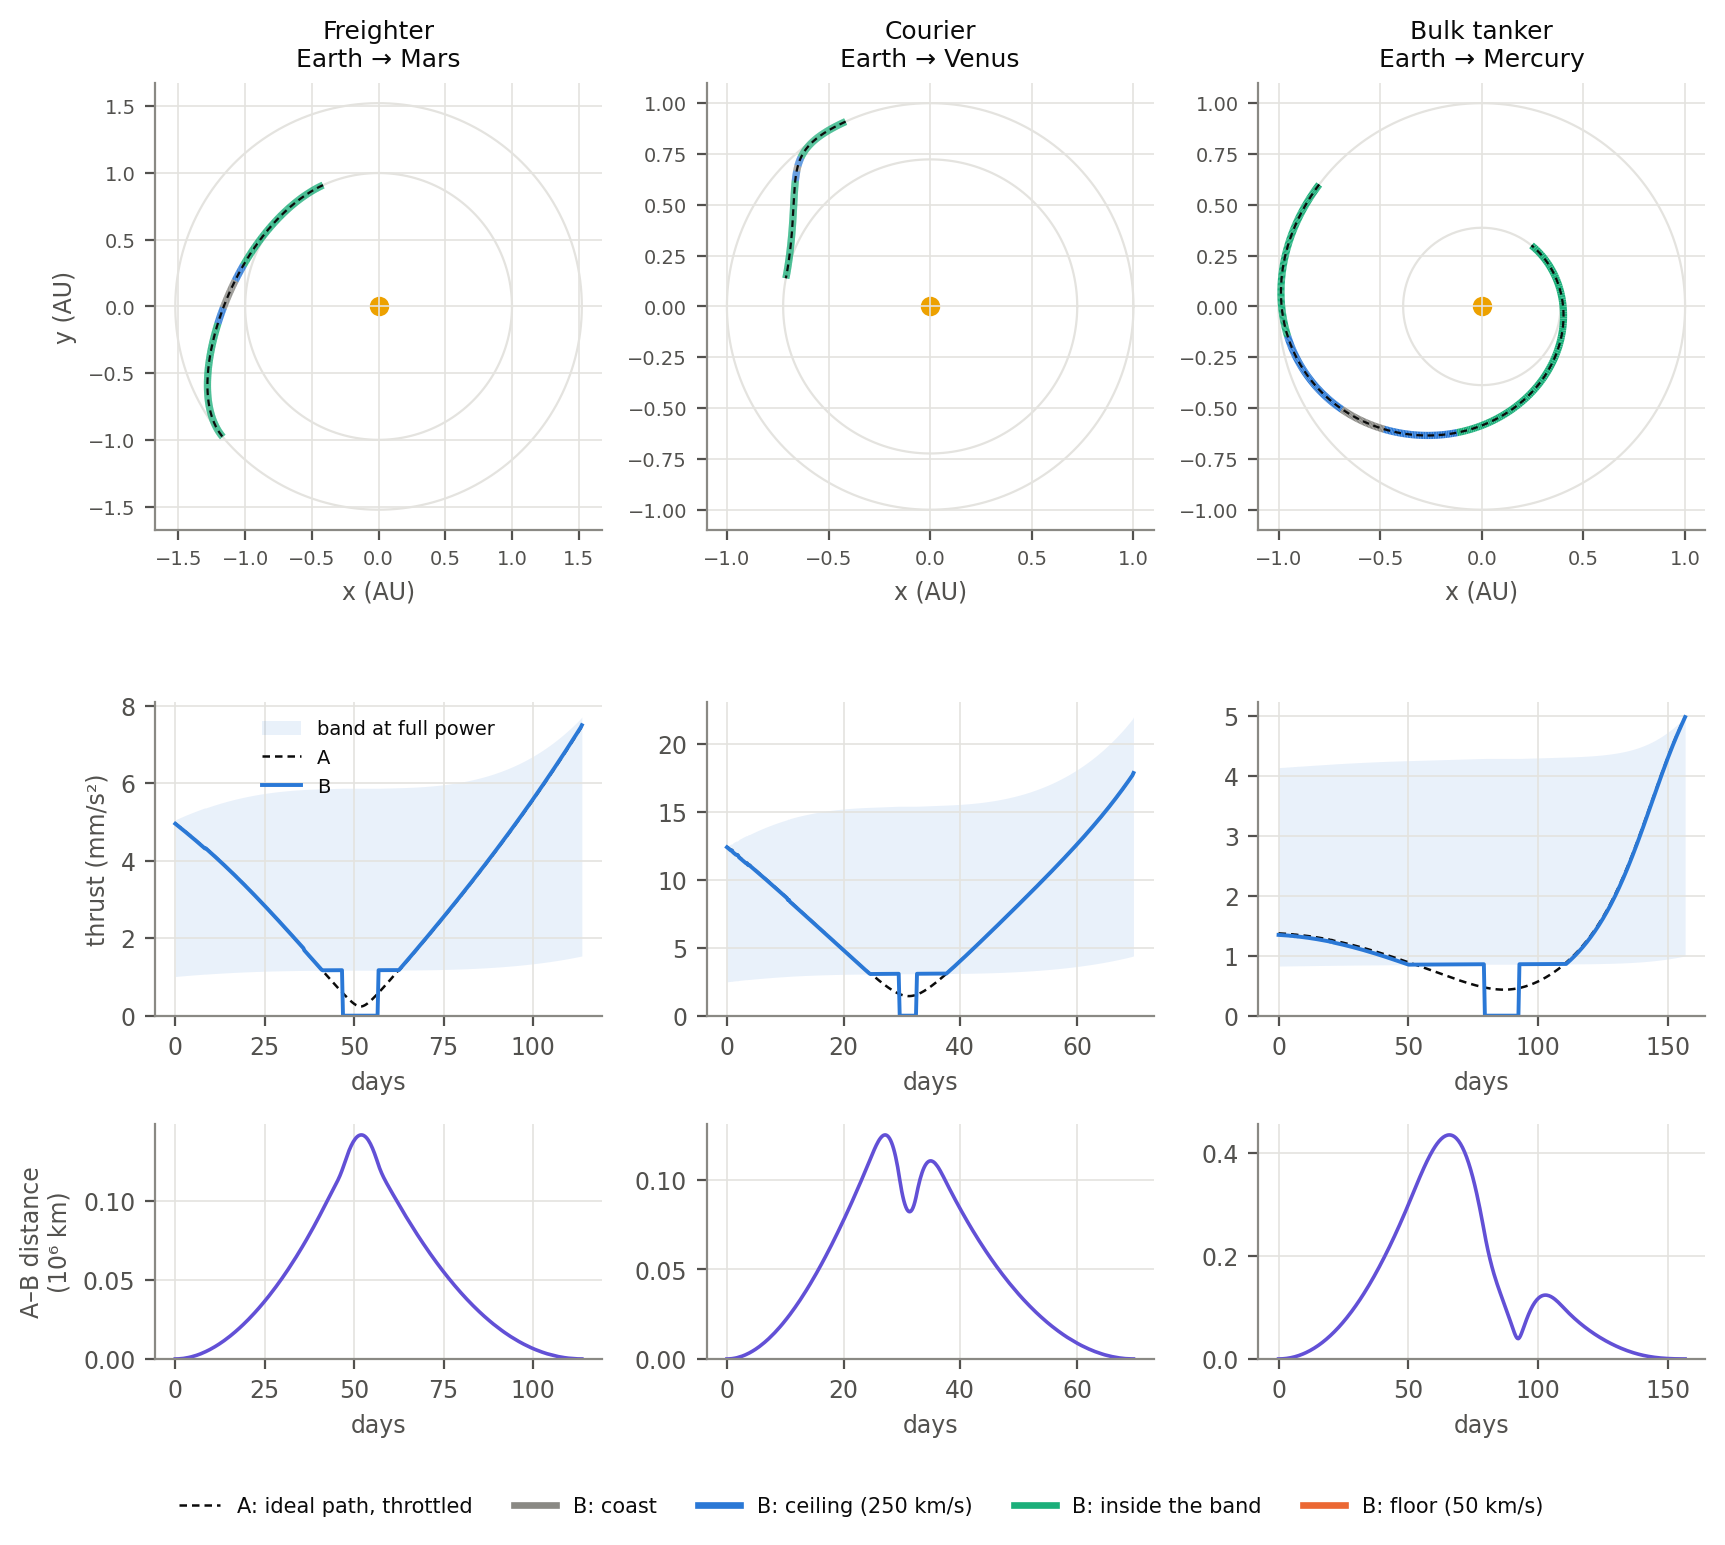
\includegraphics[width=0.92\textwidth]{paths_inner}
\caption{Inner-system examples at A's shortest full-tank time. Top: B's path coloured by arc, with A's dashed.
Middle: thrust acceleration against the band at full power (between the 250 and 50\,km/s thrusts). Bottom:
distance between the two ships. B replaces A's throttled dip with a ceiling burn, a coast and a ceiling burn.}
\label{fig:paths-inner}
\end{figure}

\begin{figure}[p]\centering
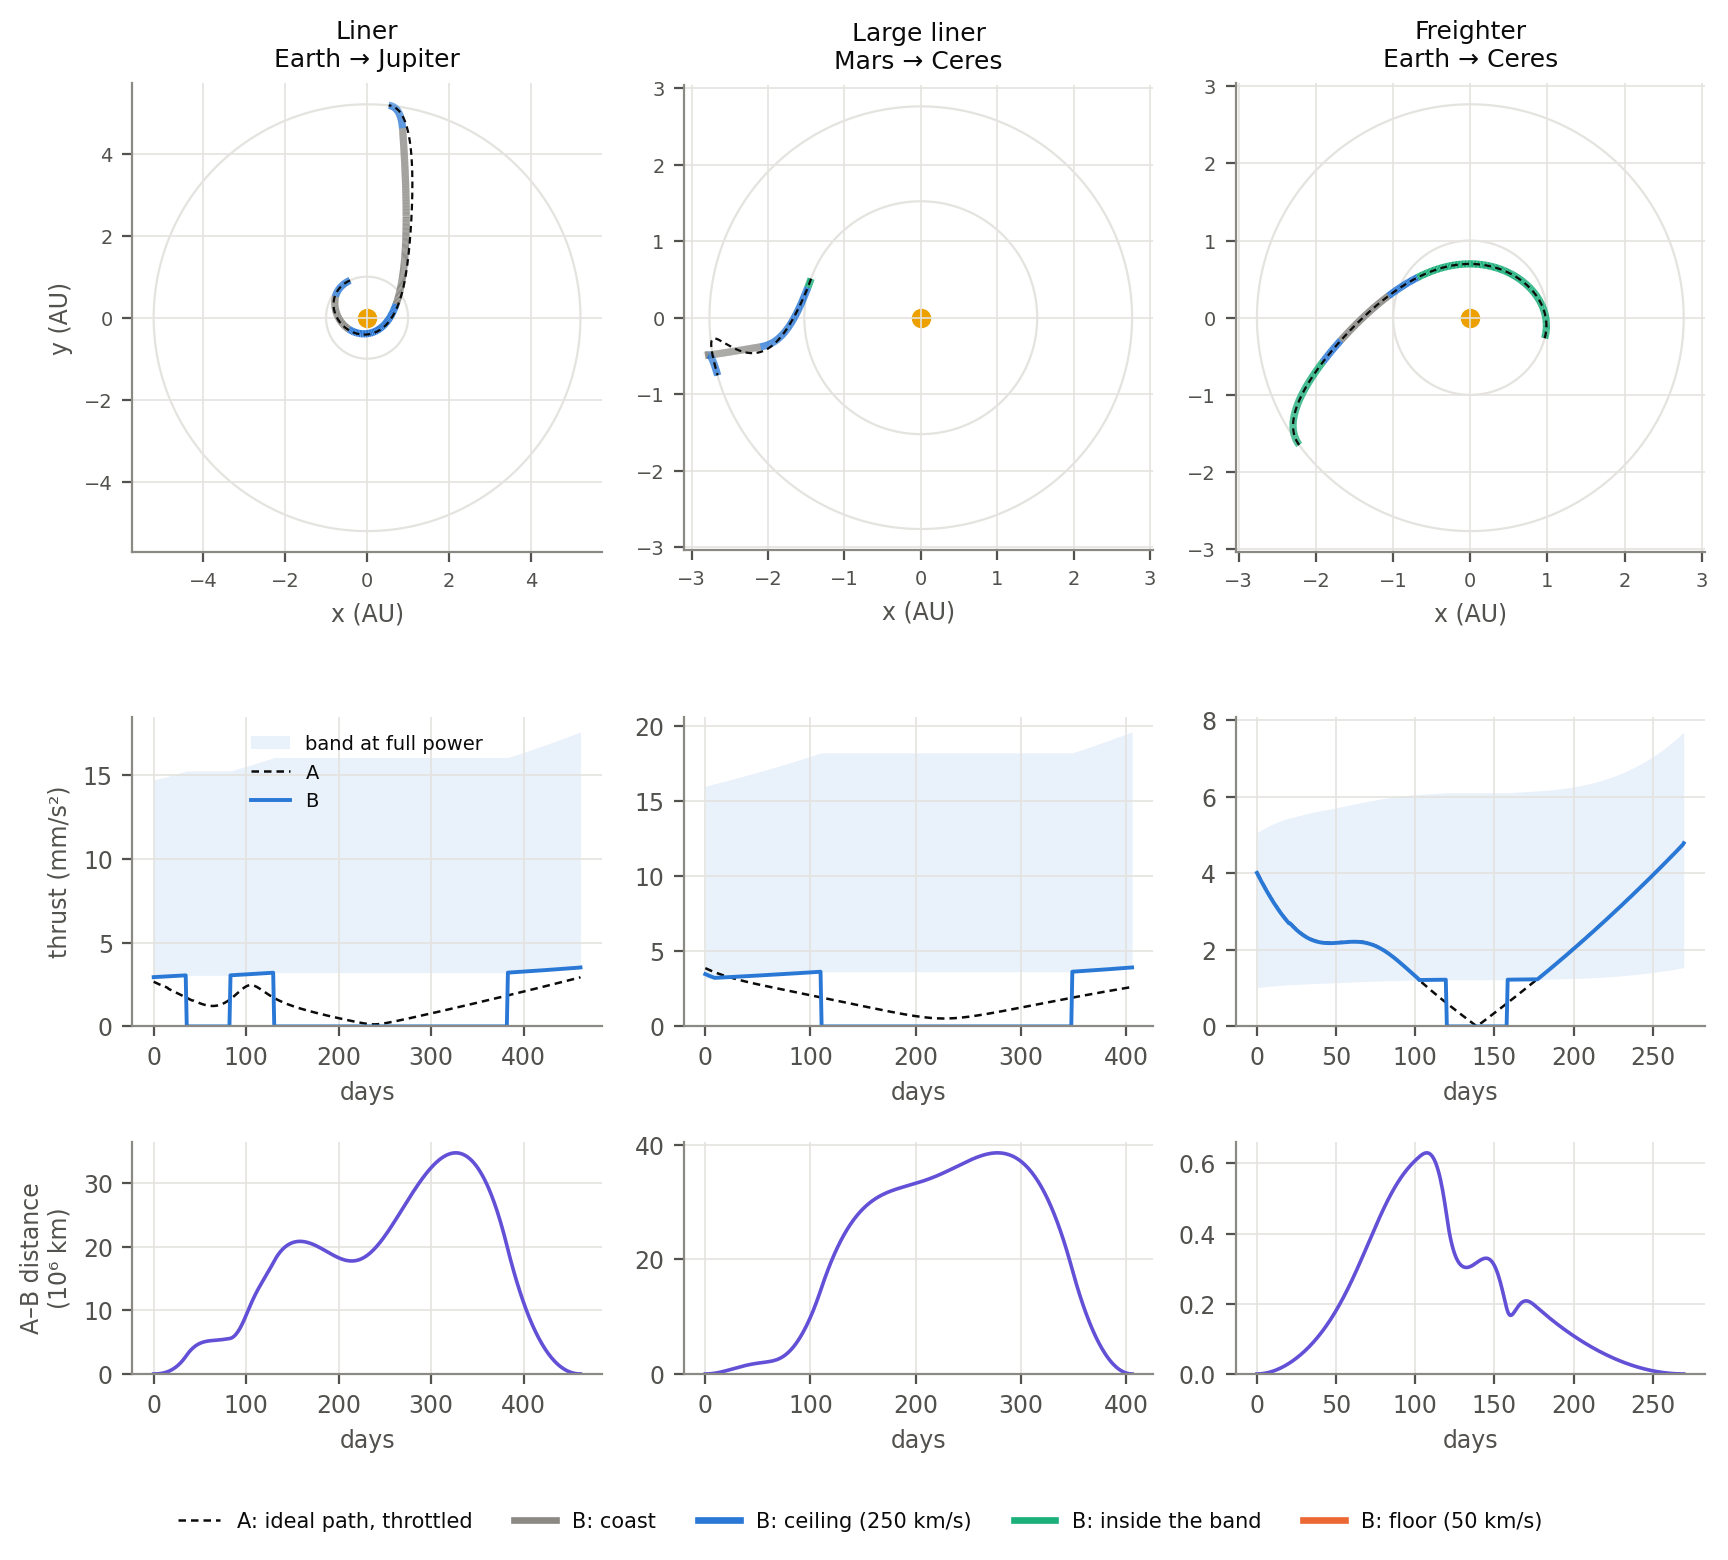
\includegraphics[width=0.92\textwidth]{paths_outer}
\caption{Outer examples. The liner to Jupiter coasts for most of its 460 days. The ships separate by 35--40 million
km on the long legs and by under a million km on the freighter's Ceres leg, which stays mostly inside the band.}
\label{fig:paths-outer}
\end{figure}

\paragraph{Shortest time on a full tank.} Table~\ref{tab:mintime} and Figure~\ref{fig:time}. A's earliest arrival is
\timeMean\% later than B's on average. The large gains, up to \timeMax\%, are on the Earth$\to$Venus and
Earth$\to$Mercury windows of the cargo hulls. There A's shortest time is limited by the 50\,km/s floor (the ideal
path asks for more thrust than the drive has near the ends), while B shifts the effort into the middle of the trip.
Every departure is flyable by both approaches. B's search fell short of A's time on \timeMiss{} of the \nBase{}
hull--departure pairs; those fly A.

\begin{table}[h]\centering\small
\caption{Earliest arrival on the standard tank. ``solver miss'': B's search returned a later time than A's, or
none; B then flies A's plan.}
\label{tab:mintime}
\tabmintime
\end{table}

\begin{figure}[h]\centering
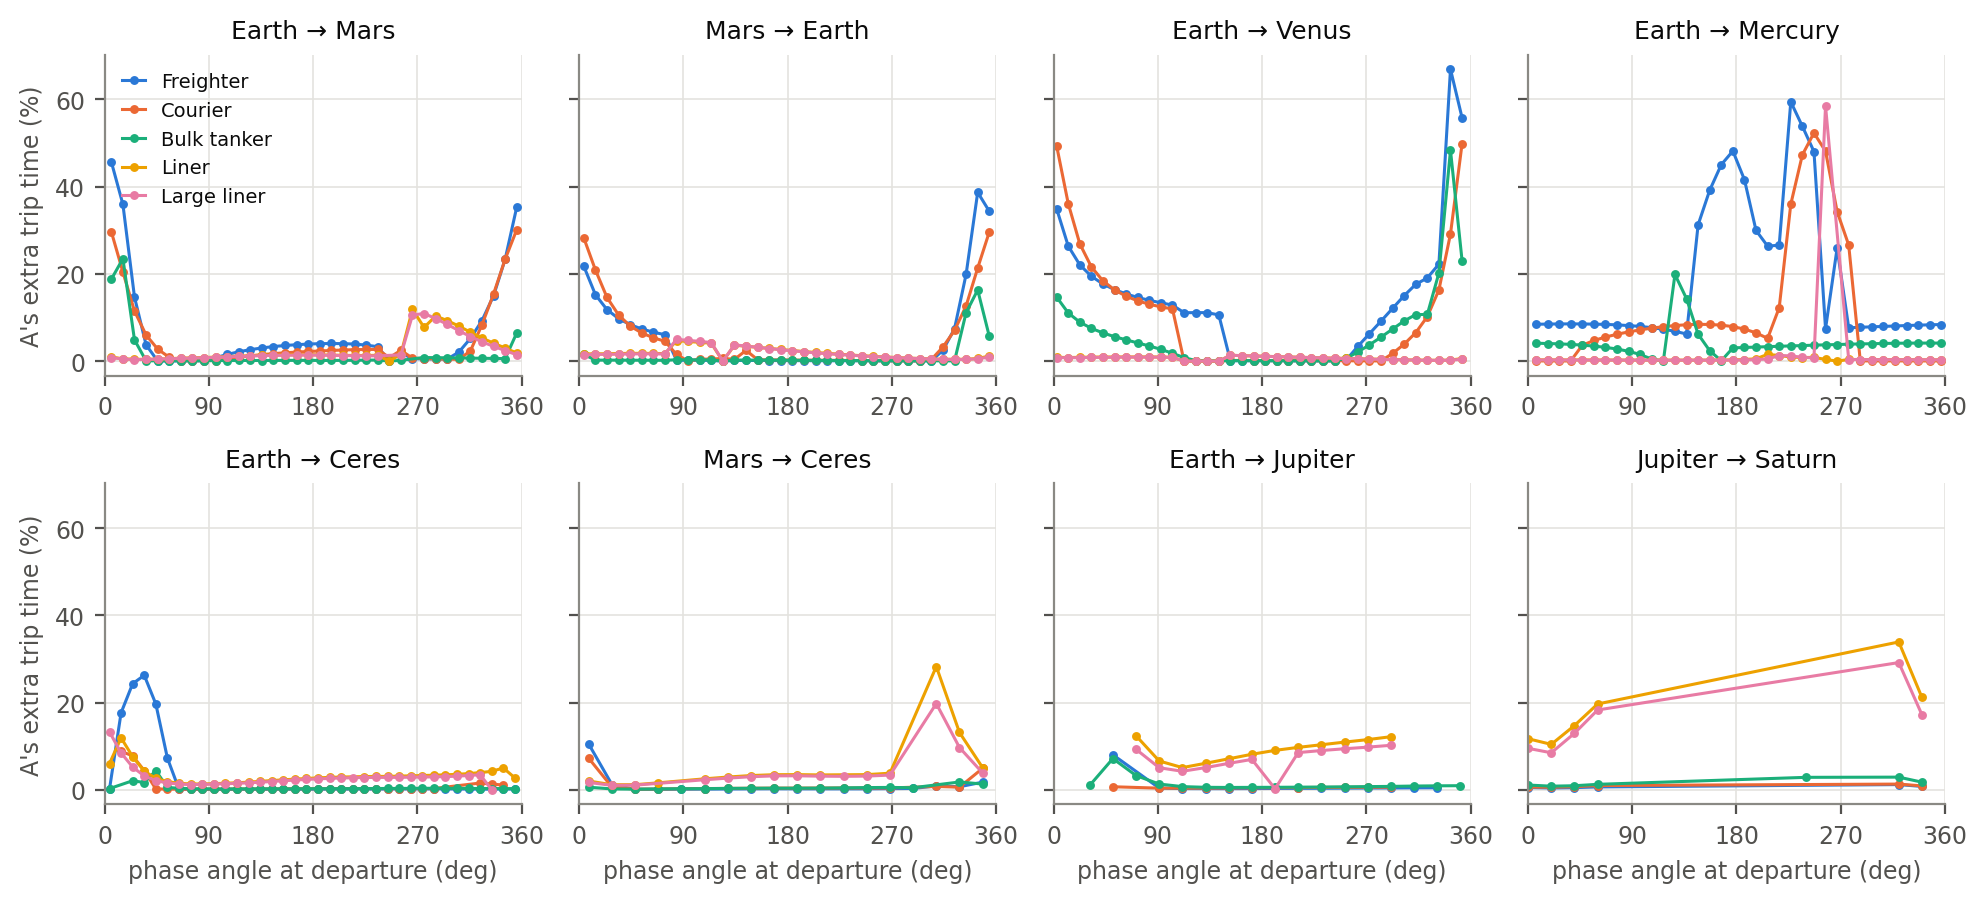
\includegraphics[width=\textwidth]{time_by_phase}
\caption{A's extra trip time on a full tank, against the departure phase angle. Solver misses are left out.}
\label{fig:time}
\end{figure}

\paragraph{Cheapest trip and tank choice.} With propellant at the game's price and time at each ship's daily cost,
the cheapest trip with A costs \econMean\% more than with B on average (Table~\ref{tab:econ}). That is 1\% for
cargo and 3\% for the liners, up to 31\%. At the optimum B flies slightly longer (by 1--3\%) and burns 4--11\% less.
The economics pick long, cheap transfers: cargo ships burn 26--41\% of a standard tank and liners about 70\%. That
is why the half-size tank is the cheapest choice for most cargo departures (Table~\ref{tab:tanks},
Figure~\ref{fig:tanks}): a smaller tank means less mass to push, and the cargo hulls seldom need more. Banded
planning makes small tanks more attractive still. It moves the liners towards the standard and half tanks, because
A's throttling penalty grows when a smaller tank makes the ship lighter and raises its thrust at the ceiling. The
best tank differs between A and B on 137 of 1170 hull--departure pairs (12\%), mostly liners.

\begin{table}[h]\centering\small
\caption{Cheapest trip (fuel bought plus daily cost times transfer time), standard tank. The $T$ and fuel ratios
are averaged over the departures where B's own optimum won.}
\label{tab:econ}
\tabeconomic
\end{table}

\begin{table}[h]\centering\small
\caption{Number of departures for which each tank size gives the cheapest trip.}
\label{tab:tanks}
\tabtanks
\end{table}

\begin{figure}[h]\centering
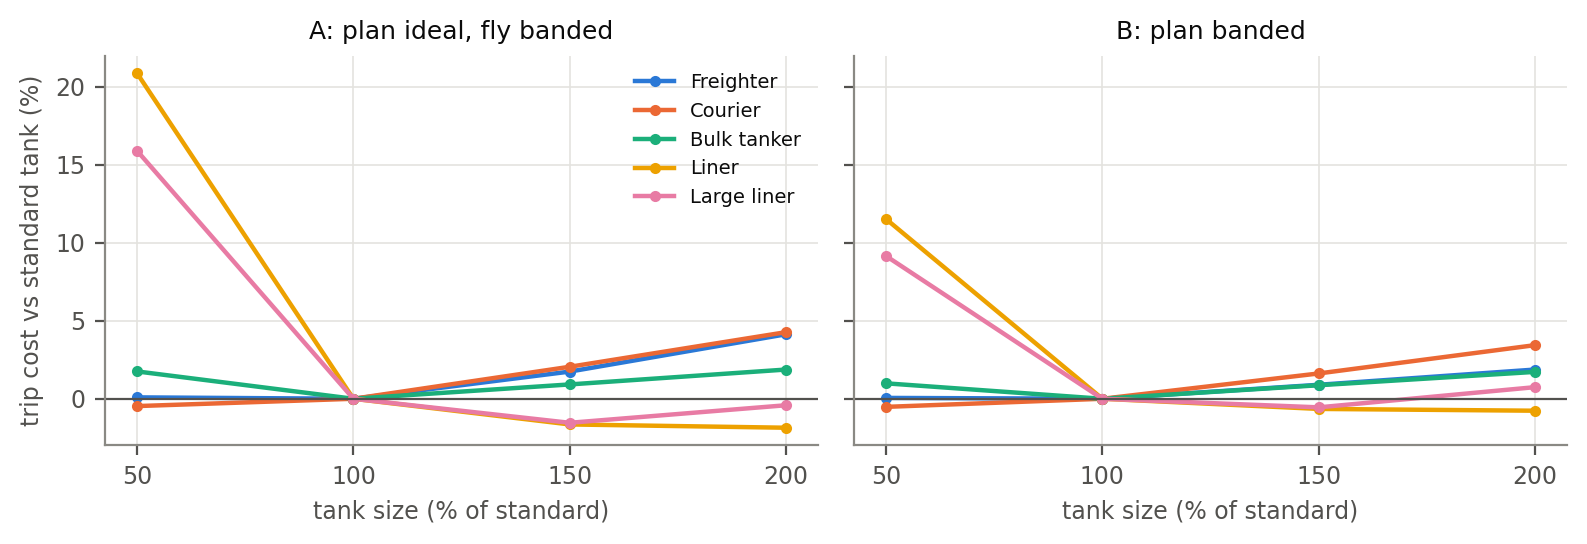
\includegraphics[width=0.85\textwidth]{tank_cost}
\caption{Mean cost of the cheapest trip by tank size, relative to the standard tank. With A, the liners pay heavily
for a half tank (20\%), because the lighter ship throttles more. With B that penalty halves.}
\label{fig:tanks}
\end{figure}

\paragraph{Speed.} Table~\ref{tab:timing} and Figure~\ref{fig:timing}, on one thread, for the \timingN{} base-tank
departures of a six-departure subset. The task is the planner's: find the earliest arrival for a full tank from
scratch. That means the ideal minimum time first, then $T$ up in 5\% steps until the approach fits, then
bisection.
\begin{itemize}
\item \textbf{Single solves.} One B solve from the ideal seed takes a median 1.1\,ms. A warm solve from a
  neighbouring time takes 0.5\,ms, faster than one ideal solve.
\item \textbf{Searches.} A full B search takes a median 9\,ms, against 3\,ms for the ideal engine and 5\,ms for A.
\item \textbf{The tail.} 10\% of B searches take more than 136\,ms. Searches that fail take 15--113\,s each,
  spent in the smoothing fallback on case after case.
\end{itemize}
Over the whole study, 18.5\% of the \bSolves{} fixed-time B solves failed. Most of those are at times where the
fuel curve has already ended (very long or infeasible), but they are what makes the sweeps slow: the study took
6.8 hours on 8--10 threads.

\paragraph{Accuracy.} Each B plan of the timing set was propagated again at a tolerance of $10^{-12}$. The arrival
miss is a median of \checkMedianM\,m, and 99\% of the plans miss by less than \checkNinetyNine\,km. One plan (a
large liner, Earth$\to$Venus) missed by 2.6 million km and 2.9\,t of propellant. Its Newton iterations alternated
between four and six switches: a short arc grazes its switching boundary, so the arc sequence, and with it the end
state, changes under a tighter tolerance. Grazing extremals like this are ill-conditioned for any switching solver.
A planner would have to re-propagate each plan and reject the ones that do not reproduce.

\begin{table}[h]\centering\small
\caption{Solve times on one thread (ms). ``Earliest arrival'' is the full search for the shortest time on a full
tank. The fixed-$T$ rows time one banded solve at the found time (from the ideal seed) and at 2\% longer (warm).}
\label{tab:timing}
\tabtiming
\end{table}

\begin{figure}[h]\centering
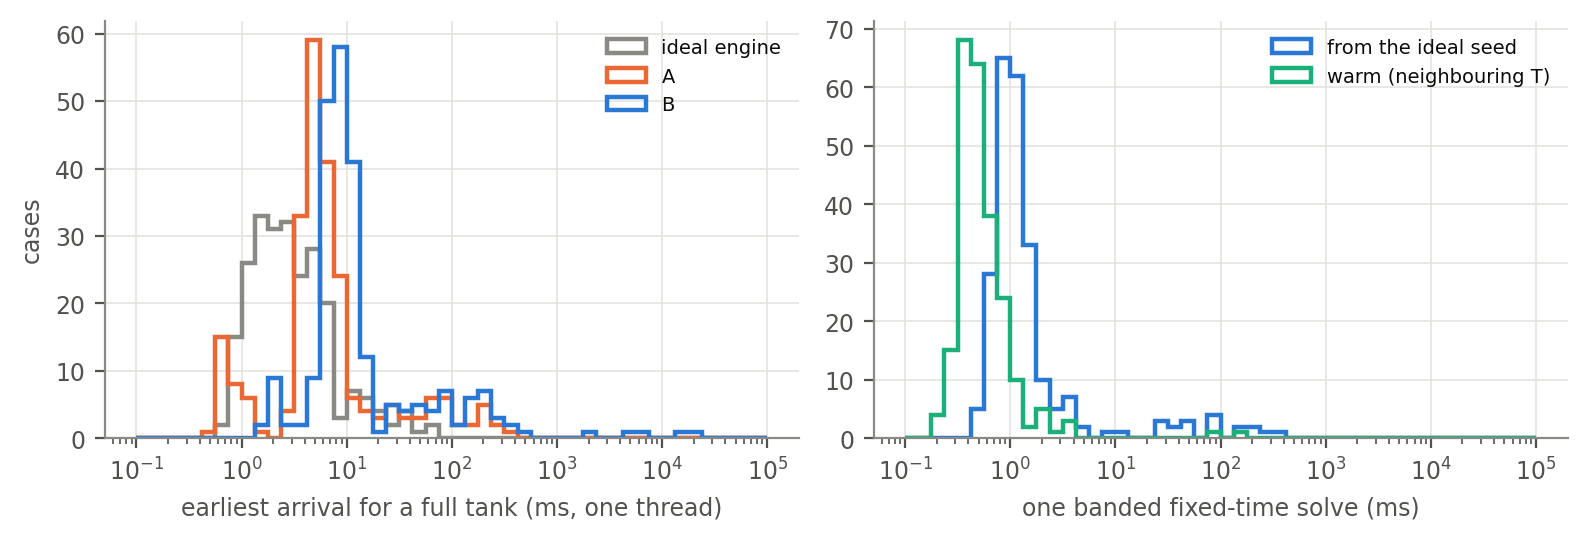
\includegraphics[width=0.9\textwidth]{timing}
\caption{Distribution of the solve times of Table~\ref{tab:timing}.}
\label{fig:timing}
\end{figure}


\clearpage
\section{Is B fit for the game?}
\label{sec:game}
\paragraph{What B buys.} For the cargo hulls, which are most of the fleet's ton-kilometres, about 1\% of propellant
and 1\% of trip cost. That is well inside the noise of the game's economy, where single runs differ by more. For
the liners, 6--7\% of propellant at their shortest times, 3\% of trip cost, and up to 30\% on bad departures. For
short inner-system windows, up to two-thirds less trip time. B also adds visible behaviour: ships that coast for a
third of the trip, and paths that differ from the ideal ones by millions of kilometres.

\paragraph{What B costs.}
\begin{enumerate}
\item \textbf{One atlas no longer serves every ship.} The ideal path does not depend on the ship, so the game
  stores one atlas of efforts and serves all hulls, loads and porkchops from it. The banded optimum depends on
  $s_0 = 2P/m_0$, so on the hull, the load and the tank. Porkchops and the planner's caches would need a dimension
  per ship state, or live solves.
\item \textbf{Live solves have a heavy tail.} The median (1\,ms per solve, 9\,ms per search) is affordable. The
  failures are not: a failing search with the smoothing fallback can block for a minute. A game solver would run
  exact-only, with a propagation budget, and fly A when it fails. On the tuning set that loses 2\% of the solved
  cases and caps a failure at about 50\,ms.
\item \textbf{Coverage and conditioning.} 18\% of fixed-time solves fail across the study, two-thirds of the
  Jupiter$\to$Saturn cases at the compared time, and rare grazing extremals do not reproduce. Each plan needs a
  verification propagation and the A fallback behind it.
\end{enumerate}

\paragraph{Recommendation.} Keep A as the game's planner, if the band is adopted at all. A is exact (the ship
flies what was planned), cheap, keeps the single atlas and the porkchops, and costs the cargo fleet about 1\%. Do
not make B the planner: the gain does not pay for per-ship atlases and an unreliable tail.

If coasting ships or the liners' 3\% matter for the game, the defensible use of B is an \emph{optional refinement
of a chosen trip}:
\begin{enumerate}
\item The dispatcher picks the trip with A, as now.
\item The departing ship then runs one warm, exact-only B solve at that transfer time (about 1\,ms, capped at
  about 50\,ms), seeded from the ideal solution.
\item The ship verifies the plan by re-propagation and flies it, or flies A if any step fails.
\end{enumerate}
The ship then burns no more than planned, often less, and liners would visibly coast. The cost is self-consistency:
porkchops and dispatch would show A's propellant, a slightly pessimistic figure, and the trip choice would ignore
B's saving. The study's cheapest trips move by only 1--3\% in $T$ when B is used, so the choice would rarely change.
A fully self-consistent banded game, with porkchops in B's numbers, would need per-hull banded atlases. On this
evidence they are not worth building.

\paragraph{The band itself.} The study also says where the band matters: wherever the thrust at 250\,km/s is high
compared with what the path needs. That is high power for the mass: the liners, and any ship made lighter, such
as one with a smaller tank or running empty. A better engine tier with a higher ceiling lowers that thrust and
shrinks A's penalty. A tier with a lower floor helps only the shortest, floor-limited inner-system trips.


\section{Limitations}
\begin{itemize}
\item Planar, Sun only, as the game. Planet-system spirals are outside the heliocentric legs; a banded spiral is
  the throttled one in closed form (the spiral's thrust is constant).
\item The ship starts and ends on the planets' states. The game's stations and launch windows add their own
  constraints.
\item The cheapest trip uses the ship's daily cost as the time value. The game's dispatch also weighs cargo value
  and passengers' time, which push towards shorter trips, where the band matters more.
\item B's coverage is not complete. Where neither the exact nor the smoothed continuation converges (long,
  coast-dominated outer transfers), B flies A's plan, which understates B's advantage there.
\item The same-time comparison is made at A's shortest full-tank time, the hardest point for A. At longer times
  both approaches burn less and the gap narrows (Figure~\ref{fig:curves}).
\item Each optimum is local. Both solvers start from the ideal path's branch; other revolution counts and branches
  were not searched.
\end{itemize}

\end{document}
